\begin{figure}[H]
    \begin{subfigure}{.49\textwidth}
        \centering
        \caption*{$u(x_1, x_2) = x_1$}
        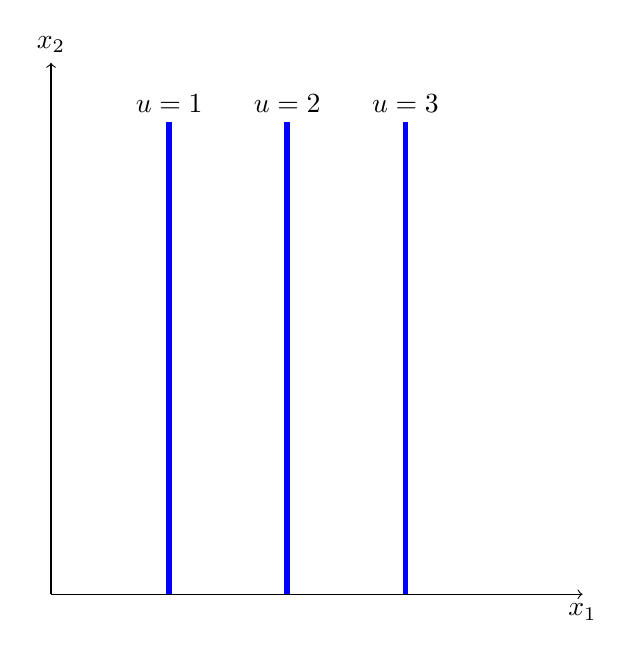
\begin{tikzpicture}[scale=1.5]
            \draw[->] (0, 0) -- (4.5, 0) node[below] {$x_1$};
            \draw[->] (0, 0) -- (0, 4.5) node[above] {$x_2$};
            \draw[domain=0:4, variable=\x, blue, line width=2pt] plot ({1}, {\x});
            \draw[domain=0:4, variable=\x, blue, line width=2pt] plot ({2}, {\x});
            \draw[domain=0:4, variable=\x, blue, line width=2pt] plot ({3}, {\x});
            \node[above] at (1,4) {$u = 1$};
            \node[above] at (2,4) {$u = 2$};
            \node[above] at (3,4) {$u = 3$};
        \end{tikzpicture}
    \end{subfigure}
    \begin{subfigure}{.49\textwidth}
        \centering
        \caption*{$u(x_1, x_2) = -2x_1 - x_2$}
        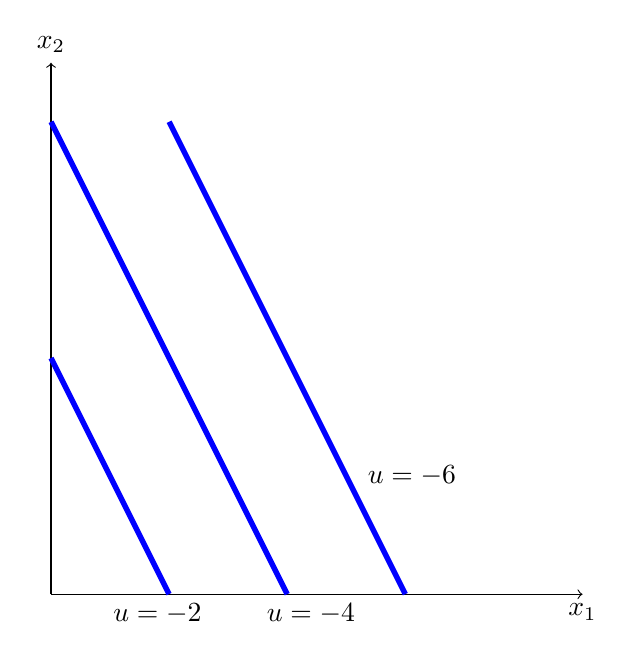
\begin{tikzpicture}[scale=1.5]
            \draw[->] (0, 0) -- (4.5, 0) node[below] {$x_1$};
            \draw[->] (0, 0) -- (0, 4.5) node[above] {$x_2$};
            \draw[domain=1:3, variable=\x, blue, line width=2pt] plot ({\x}, {-2*\x+6});
            \draw[domain=0:2, variable=\x, blue, line width=2pt] plot ({\x}, {-2*\x+4});
            \draw[domain=0:1, variable=\x, blue, line width=2pt] plot ({\x}, {-2*\x+2});
            \node[below] at (0.9,0) {$u = -2$};
            \node[below] at (2.2,0) {$u = -4$};
            \node[right] at (2.6,1.0) {$u = -6$};
        \end{tikzpicture}
    \end{subfigure}
\end{figure}
